%==============================================================================
\chapter{Novel biophysical insight from cell to whole organ: force-calcium 
to left ventricular function non-unique mapping}\label{cha:chapter8}
%==============================================================================
%
%
%
\begin{remark}{Outline}
    In this chapter, we show that the force-pCa relationship is non-uniquely mapped to LV pump function.
\end{remark}



\begin{figure}[!ht]
    \myfloatalign
    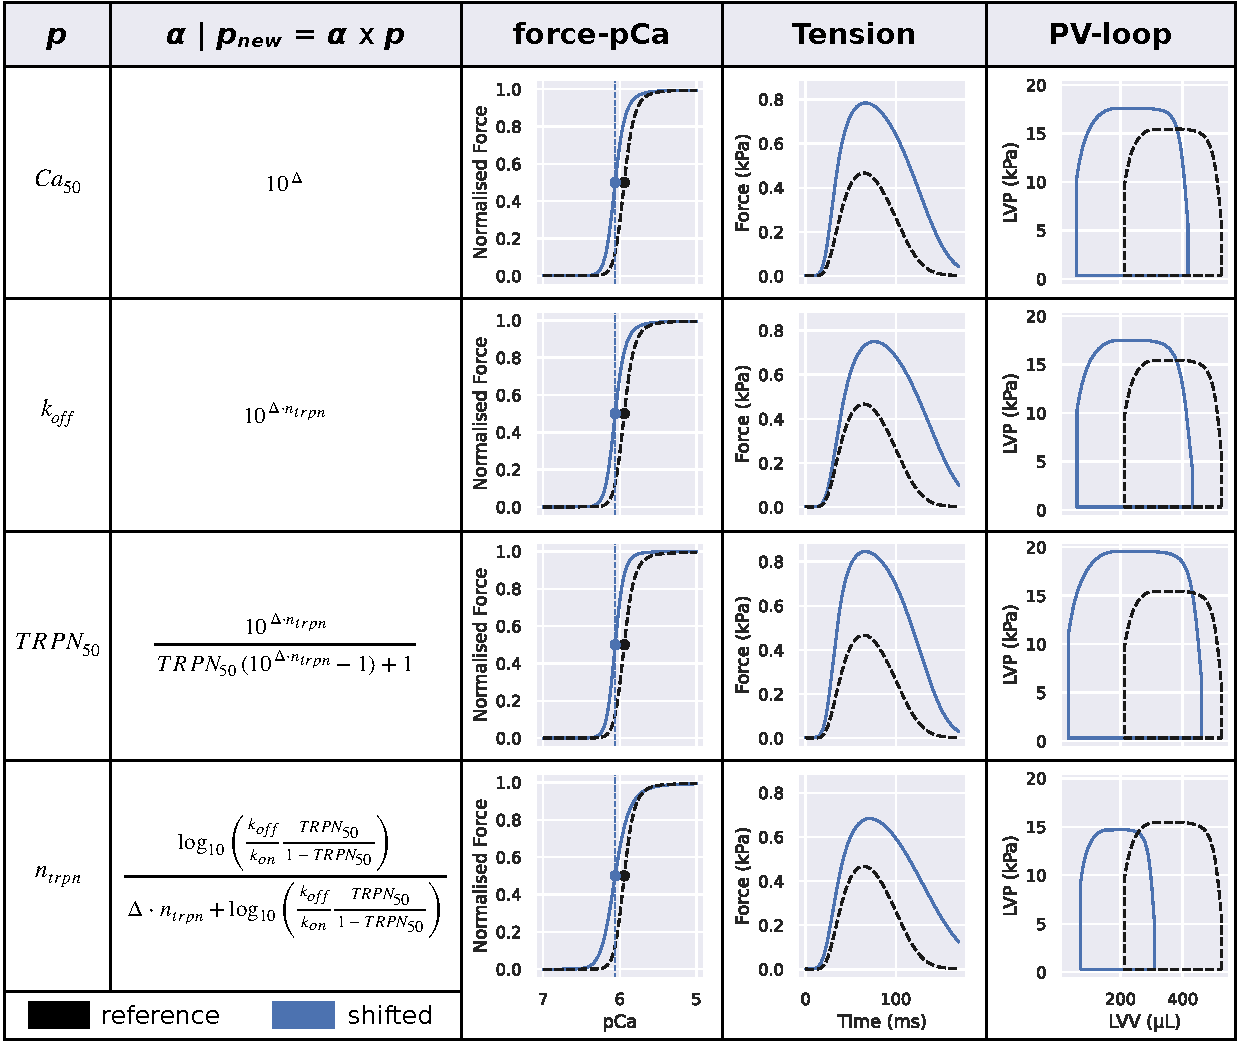
\includegraphics[width=\textwidth]{figures/chapter08/1param_pCa50_same_shift.pdf}
    \caption{Different parameters can be individually perturbed to achieve the very same shift in the force-calcium relationship. However, the performed parameter perturbation will result in different twitch transients and corresponding different pressure-volume loops. Example showing $\SI{2}{\percent}$ leftwards shift of the $\pCaf$ value.}
    \label{fig:oneparamsameshifttab}
\end{figure}


\begin{figure}[!ht]
    \myfloatalign
    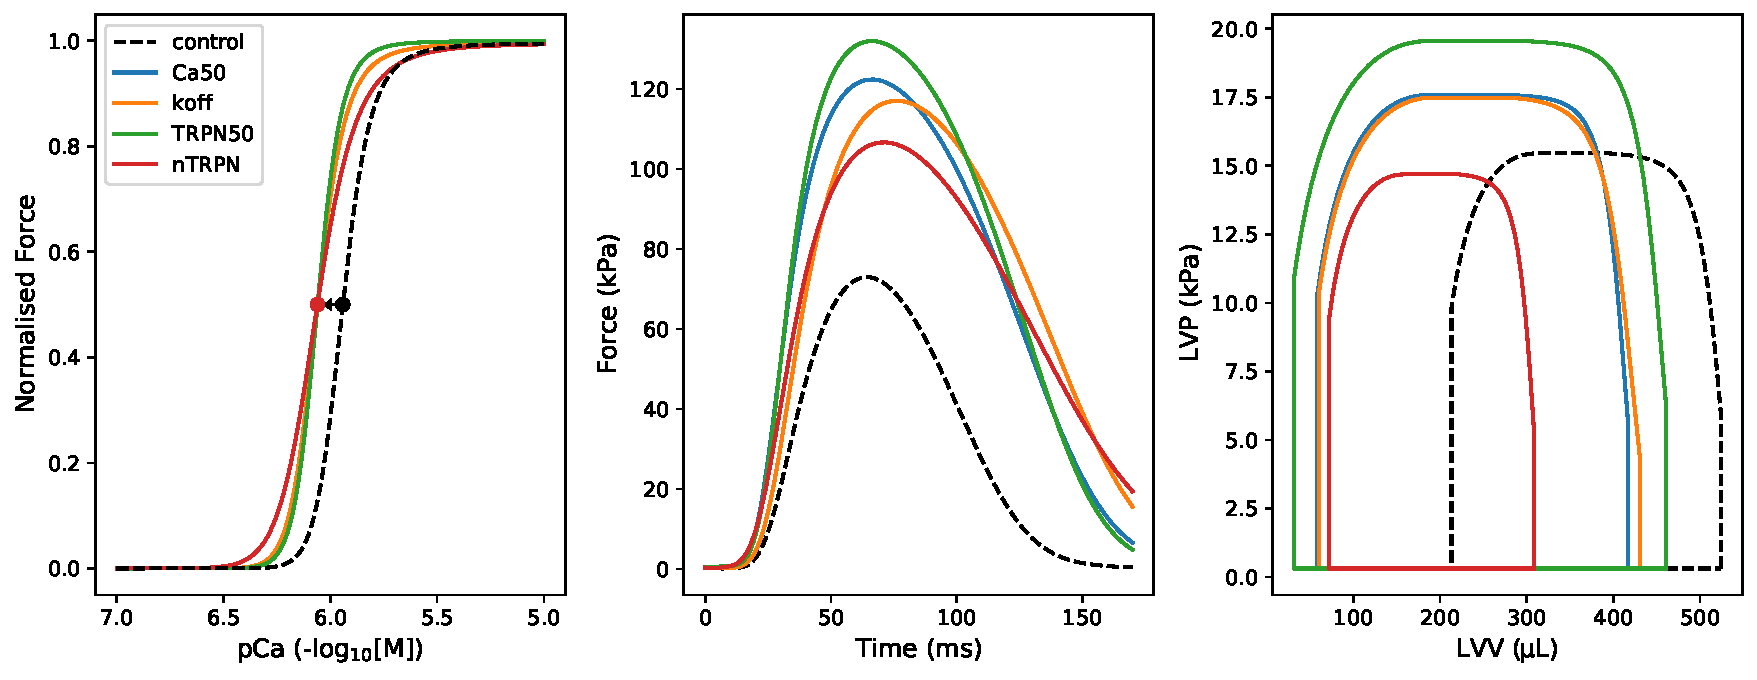
\includegraphics[width=\textwidth]{figures/chapter08/same_shift_FpCa_1param_different_Ts_and_PVloops.pdf}
    \caption{Force-pCa curves non-unique mapping. With a single-parameter \textit{ad hoc} perturbation we can achieve the exact same shift in the $\pCaf$ (although in two cases resulting in different Hill coefficients). However, the same parameter perturbations lead to very different generated force, which in turn produce different PV-loops at the whole-organ scale. Each colour represents the perturbation in the indicated parameter.}
    \label{fig:oneparamsameshift}
\end{figure}


\begin{figure}[!ht]
    \myfloatalign
    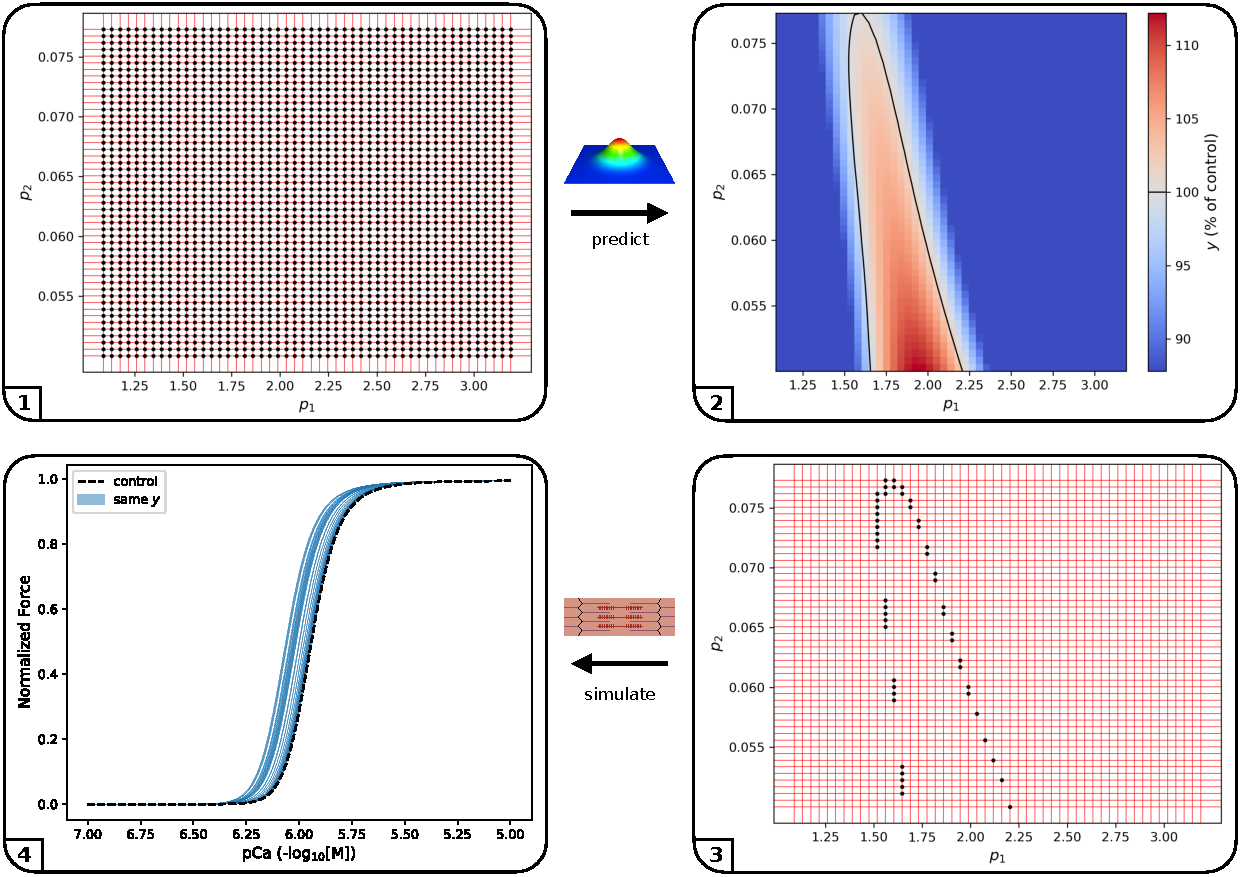
\includegraphics[width=\textwidth]{figures/chapter08/LVfeat_to_FpCa_schematic.pdf}
    \caption{LV features non-unique mapping to force-pCa curves. (1) A uniform grid of equally spaced parameters $p_1$ and $p_2$ values is mapped by the emulator into predictions of feature $y$ values. (2) An entire isoline of parameter sets $(p_1,p_2)$ sharing the same unchanged $y$ feature from reference value exists. (3) Parameters sets are extracted from the isoline using a threshold of $10^{-4}$. (4) The cell contraction model is run at each of these parameter sets to generate steady-state force-pCa curves.}
    \label{fig:gridmappingschematic}
\end{figure}


\begin{figure}[ht!]
    \myfloatalign
    \subfloat[EF feature]
    {\label{fig:twoparamssameef}
    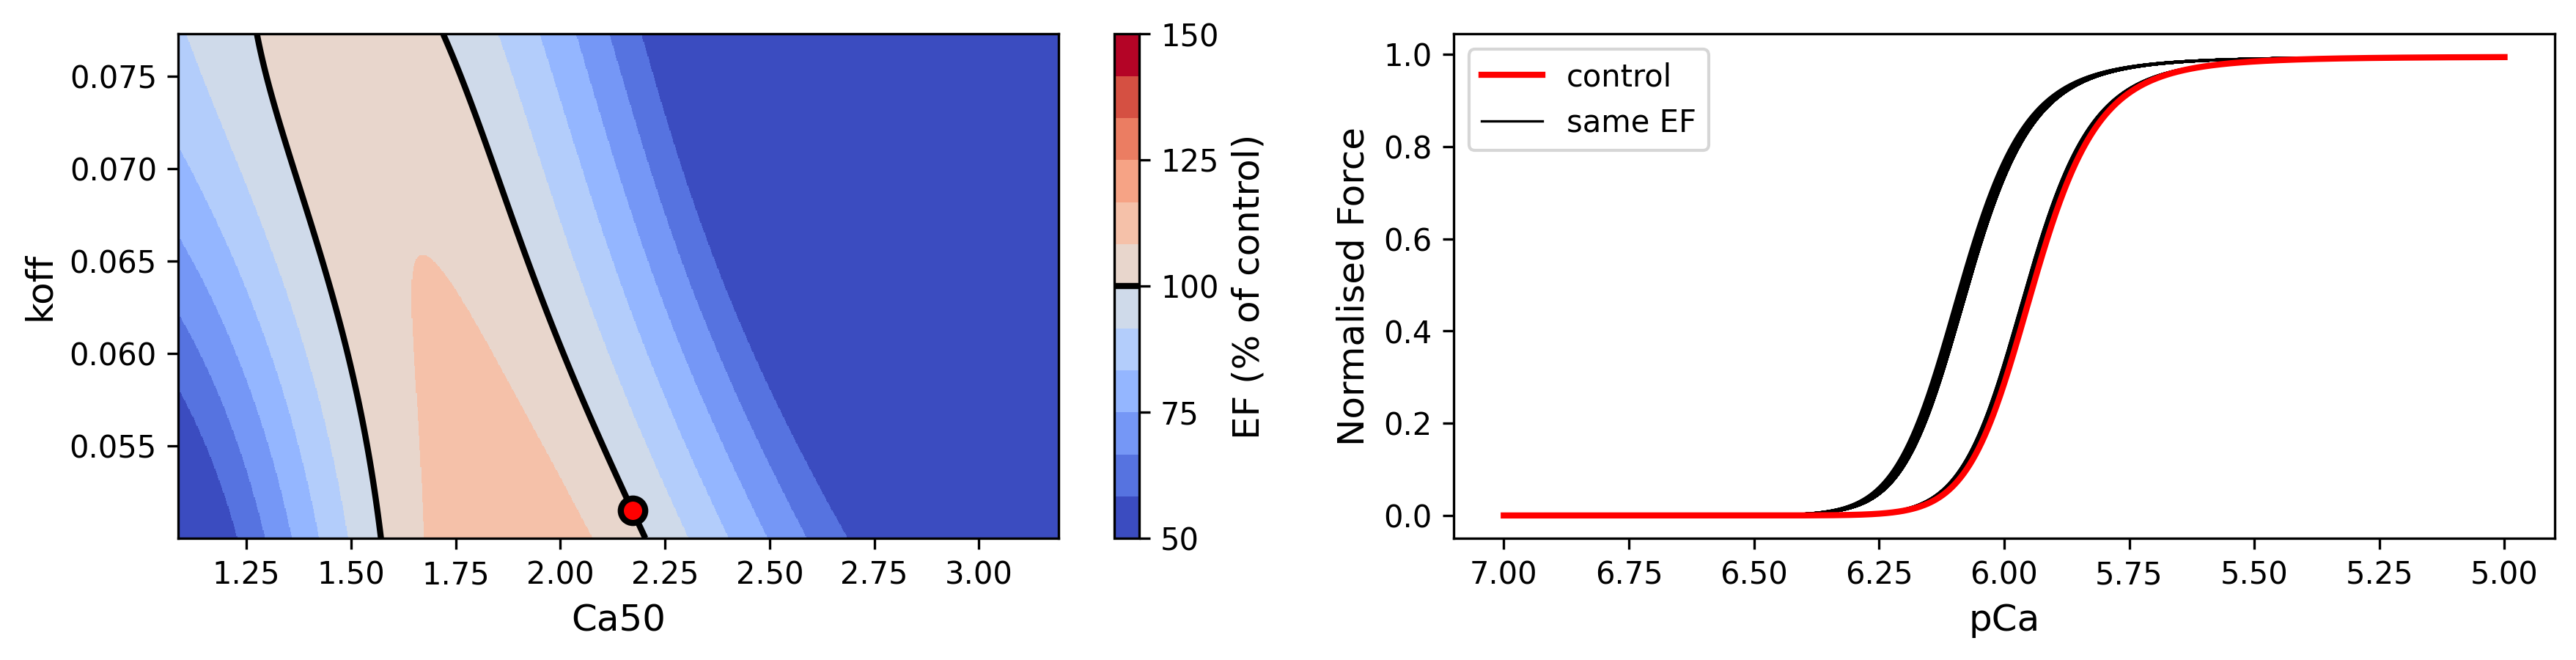
\includegraphics[width=\linewidth]{figures/chapter08/Ca50_koff_vs_EF.png}}\quad
    \subfloat[IVRT feature]
    {\label{fig:twoparamssameivrt}
    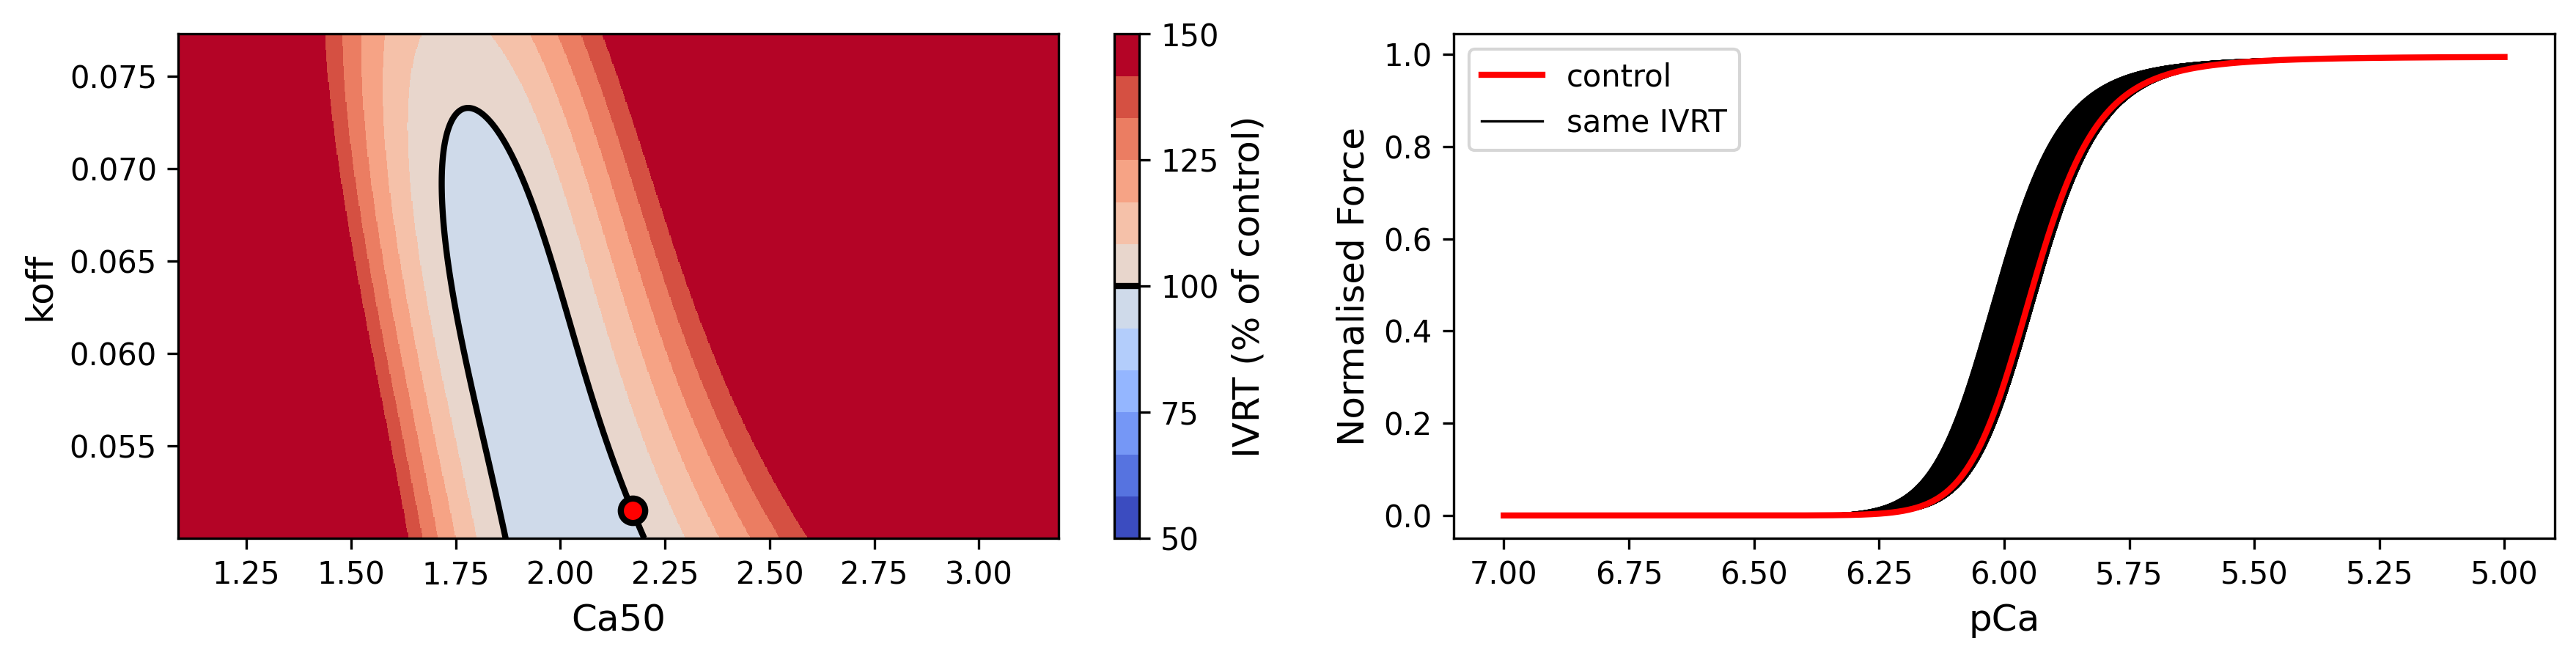
\includegraphics[width=\linewidth]{figures/chapter08/Ca50_koff_vs_IVRT.png}}
    \caption{Different Force-pCa curves are mapped to the same LV feature. A $2$-parameter grid is mapped using a trained GPE into the corresponding LV feature value for each pair of parameters within the grid. The same pairs of parameters are then used to simulate steady-state force-calcium relationships. Example showing ($\Caif,\,\koff$) parameters variations mapped into EF and IVRT features. The control parameter set is displayed as a red dot.}\label{fig:twoparamssamefeatdifffpca}
\end{figure}